\begin{frame}
  \frametitle{3D Lattice}
  \begin{columns}
    \begin{column}{0.5\textwidth}
        \begin{center}
            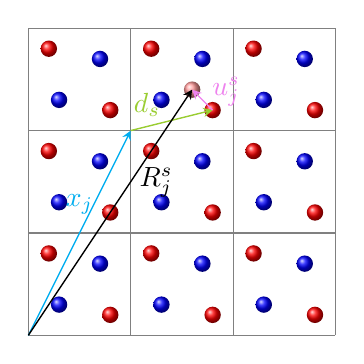
\begin{tikzpicture}
            [scale=1.3]
            \foreach \i in {0, 1, 2}{
                \foreach \j in {0, 1, 2}{
                \foreach \x/\y/\c in {0.3/0.3/blue, 0.7/0.7/blue, 0.2/0.8/red, 0.8/0.2/red}{
                    \shade[ball color=\c] (\x + \i, \y + \j) circle (0.08);
                }
                }
            }
            \foreach \i in {0, 1, 2, 3}{
                \foreach \j in {0, 1, 2, 3}{
                    \draw[thin, draw=gray] (\i, \j) -- (3, \j);
                    \draw[thin, draw=gray] (\j, \i) -- (\j, 3);
                }
            }
            % move one of the atoms
            \shade[ball color=red!40] (1.6, 2.4) circle (0.08);

            \draw[solid, draw=cyan, line width=0.5pt, ->, >=stealth]
            (0.0, 0.0) -- node[above=3pt, pos=0.5] {\textcolor{cyan}{$\boldsymbol{x}_j$}} (1.0, 2.0);

            \draw[solid, draw=YellowGreen, line width=0.5pt, ->, >=stealth]
            (1.0, 2.0) --  node[above, pos=0.2] {\textcolor{YellowGreen}{$\boldsymbol{d}_s$}} (1.8, 2.2);

            \draw[solid, draw=Violet, line width=0.5pt, ->, >=stealth]
            (1.8, 2.2) -- node[above=3pt, pos=0.5, anchor=west] {\textcolor{Violet}{$\boldsymbol{u}_{j}^s$}} (1.6, 2.4);

            \draw[solid, draw=black, line width=0.5pt, ->, >=stealth]
            (0.0, 0.0) -- node[below=5pt, pos=0.78] {$\boldsymbol{R}_{j}^s$} (1.6, 2.4);

            \end{tikzpicture}
        \end{center}
    \end{column}

    \begin{column}{0.45\textwidth}
      \begin{itemize}
      \item $\boldsymbol{x}_j$: the position of unit cell $j$
      \item $\boldsymbol{d}_s$: the equilibrum position of the atom $s$ in the cell
      \item $\boldsymbol{u}_{j}^s$: displacement from the equilibrum positon for the atom $s$ in the cell $j$
      \item $\boldsymbol{R}_{j}^s$: the position of the atom $s$ in the cell $j$
        \begin{align*}
          \boldsymbol{R}_{j}^s(t) &= \boldsymbol{x}_j + \boldsymbol{d}_s
                                + \boldsymbol{u}_{j}^s(t) \cr
                                  &= \boldsymbol{r}_j^s + \boldsymbol{u}_{j}^s(t)  \cr
          {R}_{j\alpha}^s(t) &= {r}_{j\alpha}^s + {u}_{j\alpha}^s(t) 
          \quad (\alpha= x,y,z)
        \end{align*}
      \end{itemize}
    \end{column}
  \end{columns}

  \bigskip
  The total energy can be written as
  \begin{equation*}
    E_{\text{tot}}\left(\{\boldsymbol{R}_j^s(t)\}\right) = 
    E^0_{\text{tot}}\left(\{\boldsymbol{r}_j^s\}\right) +
    \sum_{js\alpha} \frac{
      \partial E^0_{\text{tot}} % \left(\{\mathrm{r}_j^s\}\right)
    }{
      \partial {u}_{j\alpha}^s
    } {{u}_{j\alpha}^s} +
    {1\over2} \sum_{\substack{js\alpha \\ kt\beta}}
    \frac{
      \partial^2 E^0_{\text{tot}} % \left(\{\mathrm{r}_j^s\}\right)
    }{
      \partial {u}_{j\alpha}^s
      \partial {u}_{k\beta}^t
    } \tikzmark{IFC}
    {{u}_{j\alpha}^s} {{u}_{k\beta}^t}
    + \ldots
       % \quad (\alpha,\beta = x,y,z)
  \end{equation*}
  \vspace{-6pt}

  % \begin{tikzpicture}
  %   [overlay, remember picture]
  %   \node[below right=12pt of IFC, align=center]
  %   (IFC_NOTE) {
  %     $C_{s\alpha, t\beta}(k - j)$
  %   };
  % \end{tikzpicture}

  \begin{itemize}
  \item The expression is exact if we take all the orders in the expansion.
  \item All the derivatives are taken at the equilibrium positions
    $\{\boldsymbol{r}_j^s\}$, i.e. $
    \frac{
      \partial E^0_{\text{tot}}
    }{
      \partial
      {u}_{j\alpha}^s
    }=0$. 
  \item Harmonic approximation: truncated at \emph{second} order.
  \end{itemize}
\end{frame}